\documentclass{article}
%\documentclass{standalone}

\usepackage[active,pdftex,tightpage]{preview}
\usepackage{tikz}

\definecolor{logoYellow}{RGB}{255, 249, 232}
\definecolor{blGreen}{rgb}{.2,.7,.3}
\definecolor{darkRed}{rgb}{.3,0,0}
\newcommand{\sovn}[1]{\color{yellow!20!logoYellow}{{\textbf{#1}}}}

\newcommand{\mybox}[1]{\colorbox{grred!10!darkRed}{\parbox{2mm}{\sovn{#1}}}}

\newcommand{\circled}[1]{{\mybox{#1}}}

\PreviewEnvironment{tikzpicture}

% remove "[demo]" if you want include actual image!!!
\usepackage{graphicx}

\usepackage{tikz}

% LaTeX Overlay Generator - Annotated Figures v0.0.1
% Created with http://ff.cx/latex-overlay-generator/

\definecolor{postBkgColor}{rgb}{.95,.85,.95}
\definecolor{postCommentBkgColor}{rgb}{.85,.85,.95}

\definecolor{grammarArrowColor}{rgb}{.85,.85,.45}

\colorlet{brred}{brown!53!red}
\colorlet{grred}{grammarArrowColor!40!red!60}

\definecolor{logoRed}{rgb}{.3,0,0}
\definecolor{logoPeach}{RGB}{255, 159, 102}
\definecolor{logoCyan}{RGB}{66, 206, 244}
\definecolor{logoBlue}{RGB}{4, 2, 25}

\colorlet{lplr}{logoPeach!40!logoRed}

%%%%%%%%%%%%%%%%%%%%%%%%%%%%%%%%%%%%%%%%%%%%%%%%%%%%%%%%%%%%%%%%%%%%%%
%\annotatedFigureBoxCustom{bottom-left}{top-right}{label}{label-position}{box-color}{label-color}{border-color}{text-color}
\newcommand*\annotatedFigureBoxCustom[8]{\draw[#5,thick,rounded corners] (#1) rectangle (#2);\node at (#4) [fill=#6,thick,shape=circle,draw=#7,inner sep=2pt,font=\sffamily,text=#8] {\textbf{#3}};}
%\annotatedFigureBox{bottom-left}{top-right}{label}{label-position}
\newcommand*\annotatedFigureBox[4]{\annotatedFigureBoxCustom{#1}{#2}{#3}{#4}{lplr}{grred!30!black}{brred}{brred!20}}
\newcommand*\annotatedFigureText[4]{\node[draw=none, anchor=south west, text=#2, inner sep=0, text width=#3\linewidth,font=\sffamily] at (#1){#4};}
\newenvironment {annotatedFigure}[1]{\centering\begin{tikzpicture}
    \node[anchor=south west,inner sep=0] (image) at (0,0) { #1};\begin{scope}[x={(image.south east)},y={(image.north west)}]}{\end{scope}\end{tikzpicture}}
%%%%%%%%%%%%%%%%%%%%%%%%%%%%%%%%%%%%%%%%%%%%%%%%%%%%%%%%%%%%%%%%%%%%%%

\begin{document}

    \begin{figure}[h!t]

        \begin{annotatedFigure}
            {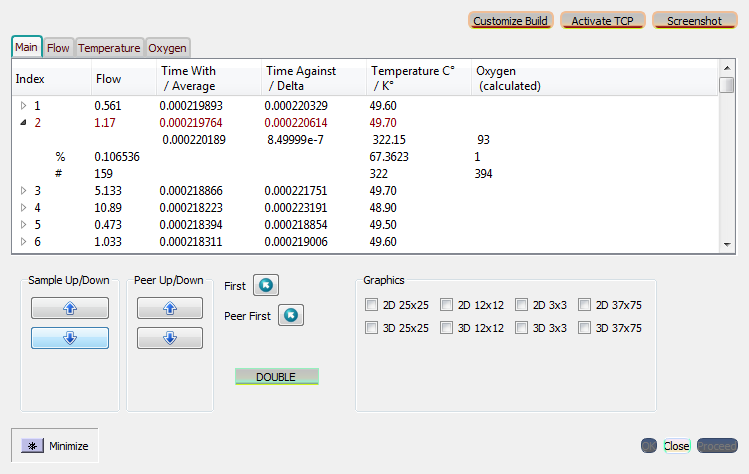
\includegraphics[scale=1]{expand.png}}
            
  \node [text width=7.3cm,align=justify,fill=logoCyan!20, draw=logoBlue, 
  draw opacity=0.5,line width=1mm, fill opacity=0.9]
   at (0.74,0.465){\textbf{Using a ``tree widget" (a two-layer spreadsheet), 
  instead of a conventional spreadsheet, allows the Dataset Application to 
  distinguish primary values (those measured directly by physical devices 
  and experimental equipment) from intermediate values calculated via algorithms.}};
              
            \annotatedFigureBox{0.01,0.6}{0.75,0.77}{1}{0.75,0.6}
            
  \node [text width=7.8cm,align=justify,fill=logoCyan!20, draw=logoBlue, 
  draw opacity=0.5,line width=1mm, fill opacity=0.9]
   at (0.23,0.475){\textbf{In addition, nested rows can 
   display supplemental infomation, such as data values' 
   rank (\circled{3}) and percentage (\circled{2}) 
   (on the scale of the least to greatest 
   value) relative to all other values for each statistical parameter.}};
              
            \annotatedFigureBox{0.015,0.65}{0.1,0.69}{2}{0.1,0.69}
            \annotatedFigureBox{0.015,0.62}{0.1,0.648}{3}{0.1,0.625}                        
            
            
            
            %bl
      %      \annotatedFigureBox{0.222,0.284}{0.3743,0.4934}{B}{0.3743,0.4934}%tr
      %      \annotatedFigureBox{0.555,0.784}{0.6815,0.874}{C}{0.555,0.784}%bl
      %      \annotatedFigureBox{0.557,0.322}{0.8985,0.5269}{D}{0.8985,0.5269}%tr
  

  
        \end{annotatedFigure}

   %     \caption{Expanded Sample (A)}
    %    \label{fig:teaser}

    \end{figure}

\end{document}
